\chapter{基于黑板调度的多智能体协同推理机制}
\label{chp:system}

PlanGraph 的图推理求解过程涉及规划、检索、编码、验证和反馈修复等多个阶段。第三章重点讨论规划反馈如何形成图推理求解方法，本章进一步研究多个智能体在同一求解链路中如何保持状态一致、定位错误来源并完成有界恢复。图推理通常包含结构解析、约束识别、算法选择、代码执行和答案格式化等环节，任一阶段的不稳定都可能影响最终结果；若仅依赖多个智能体自由对话，整体流程容易出现职责混杂、上下文覆盖、错误来源不清和失败后无序重试等问题。因此，本章关注的是面向多阶段图推理过程的黑板调度协同推理机制。

PlanGraph 将多智能体协作抽象为由主流程调度器、角色智能体、共享黑板和共享缓存构成的受控协同过程：主流程调度器负责阶段推进和回退决策，角色智能体负责局部任务生成，共享黑板负责维护状态和事件，共享缓存负责保存规划、检索、候选程序和验证反馈等可复核阶段结果。围绕状态一致性、错误归因和有界恢复三个目标，本章依次说明协同状态建模、协同调度、反馈恢复、运行记录诊断以及协同推理机制验证等内容。

\section{研究问题定义}

从协同推理视角看，本文关注多个角色智能体在统一控制下完成一条可追溯的图推理求解链路。给定自然语言图推理任务，PlanGraph 依次产生任务表示、规划结果、检索知识、候选程序、执行反馈和最终答案。该过程需要解决三个问题：多个智能体之间如何维护一致的共享状态，执行失败后如何判断错误更可能来自任务解析、规划约束、检索知识、程序实现还是答案格式，以及错误定位结果如何转化为局部修复、补充检索或上游回退等有界恢复动作。

因此，PlanGraph 在运行时固定三类约束：状态只通过黑板和缓存版本更新，失败只根据错误类型和剩余预算回退，实验日志必须保留阶段产物及其依赖关系。这样可以减少角色智能体在多轮协作中覆盖前序结论，也使稳定性分析和结果复核能够追溯到具体阶段。

为描述上述状态管理问题，本文将第 $t$ 个阶段的共享黑板状态抽象为：
\begin{equation}
B_t=\{Q,S,P,K,C,E,F,A\}
\end{equation}
其中，$Q$ 表示原始自然语言问题，$S$ 表示运行期结构化任务表示，与第\ref{chp:method}章中的任务描述 $T$ 对应，$P$ 表示规划结果，$K$ 表示规划引导检索得到的知识集合，$C$ 表示候选求解程序，$E$ 表示执行验证结果，$F$ 表示反馈修复信息，$A$ 表示最终答案。该抽象使多智能体协同过程可以被统一理解为围绕黑板状态 $B_t$ 的读写与转移：不同智能体只更新与自身职责相关的状态分量，主流程调度器则根据当前状态和验证反馈决定下一阶段动作。

基于上述目标，PlanGraph 将协同推理过程建模为以主流程调度器为中心、以共享黑板和共享缓存链为支撑的多智能体协同框架。PlanGraph 接收自然语言问题和图结构输入，在输出最终答案的同时，保留对应的阶段结果、运行日志和恢复记录。该设计通过明确的职责划分，把规划反馈方法落实为可控制、可记录的执行过程。

图推理任务需要在多个阶段之间稳定传递任务表示、规划、检索知识、候选程序和验证反馈。黑板调度可以集中维护共享状态，同时通过事件和缓存索引保留错误来源及恢复记录，因而更适合本文对可追踪、可恢复和可复现实验过程的要求。

\section{基于共享黑板的协同状态建模机制}

多智能体协同推理的首要问题是状态一致性。若不同角色智能体仅通过自然语言上下文传递信息，规划结果、检索知识和执行反馈容易在多轮调用中被覆盖或重新解释。为此，PlanGraph 将协同过程建模为围绕共享黑板状态的受控读写过程，通过角色智能体职责划分、黑板状态表示和事件记录约束各阶段的信息边界。

\subsection{角色智能体的职责划分}

如果让不同角色智能体仅通过自然语言彼此对话，并由模型自行决定何时规划、检索和修复，图推理流程容易出现控制流不稳定。典型问题包括角色智能体职责重复，例如规划智能体和编码智能体都重新解释任务；也包括失败后回退位置不清，例如程序执行失败后难以判断应回到规划、检索还是编码阶段。PlanGraph 因此将全局流程交由主流程调度器统一管理，各角色智能体只负责本阶段的局部任务。

图\ref{fig:system_architecture}给出了 PlanGraph 的总体架构。自上而下，系统可划分为输入与任务建模层、主流程调度层、多智能体执行层以及共享状态管理层。输入与任务建模层负责接收自然语言问题和图结构信息；主流程调度层负责推进阶段、检查状态并决定失败后的恢复动作；多智能体执行层包含问题智能体、规划智能体、检索智能体、编码智能体和推理智能体；共享状态管理层则维护黑板事件、共享缓存、知识条目和执行反馈。该架构强调运行期控制关系，即调度器如何组织各角色智能体协同、如何保存阶段状态，以及框架如何在失败后进入受控恢复路径。

\begin{figure}[htbp]
\centering

\includegraphics[width=0.98\textwidth]{figures/paper/SystemArchitecture.pdf}
\caption{PlanGraph 总体架构}
\label{fig:system_architecture}
\end{figure}

在具体运行中，调度器维护当前样例的运行状态、已有缓存项以及剩余恢复预算。各角色智能体被调用时，只读取本阶段所需的信息。例如，规划智能体读取结构化任务表示，检索智能体读取规划结果和任务标签，编码智能体读取规划与知识条目，推理智能体读取候选程序和验证反馈。阶段任务完成后，智能体将生成结果写入共享缓存，并在共享黑板中记录相应事件。角色智能体之间不直接互相调用，也不各自维护复杂的私有上下文；协作关系由调度器和黑板统一管理。

\subsection{角色智能体的读写边界}

共享黑板需要配合明确的访问边界使用。为避免多智能体协同中的职责重叠和状态覆盖，PlanGraph 为不同角色智能体和功能模块设置相对稳定的读写边界。问题智能体主要负责把原始问题写入结构化任务表示，规划智能体在此基础上写入规划和约束标签，检索智能体只根据任务表示和规划结果补充知识，编码智能体读取规划与知识生成候选程序，推理智能体则根据执行反馈修复候选程序。调度器读取黑板状态、缓存索引和错误反馈，并据此决定下一阶段动作。

\begin{table}[htbp]
\centering
\small
\caption{角色智能体读写边界}
\label{tab:agent_read_write}
\renewcommand{\arraystretch}{1.15}
\begin{tabularx}{\textwidth}{
>{\raggedright\arraybackslash}p{2.3cm}
>{\raggedright\arraybackslash}p{2.8cm}
>{\raggedright\arraybackslash}p{2.8cm}
>{\raggedright\arraybackslash}X}
\toprule
角色/模块 & 主要读取状态 & 主要写入状态 & 边界约束 \\
\midrule
问题智能体 & $Q$ & $S$ & 只负责结构化任务表示，不生成求解程序 \\
规划智能体 & $S$ & $P$ & 生成算法级规划和约束标签，不直接调用图算法 \\
检索智能体 & $S,P,F$ & $K$ & 根据规划和反馈召回知识，不改写规划内容 \\
编码智能体 & $S,P,K$ & $C$ & 根据规划和知识生成候选程序，不重新解释任务类型 \\
验证模块 & $S,P,C$ & $E$ & 执行候选程序并产生验证结果，不修复程序 \\
推理智能体 & $P,K,C,E$ & $F,C$ & 根据错误反馈局部修复，不覆盖上游缓存 \\
调度器 & $B_t,E,F$ & 阶段状态 & 决定阶段推进、回退和失败退出，不生成局部内容 \\
\bottomrule
\end{tabularx}
\end{table}

读写边界把黑板状态约束为阶段状态记录。每个角色智能体或模块只能围绕自身职责更新对应状态分量，从而减少规划被编码阶段重新解释、检索知识被修复阶段覆盖、验证反馈在多轮调用中丢失等问题。状态一致性既依赖缓存保存结果，也依赖角色智能体和功能模块对黑板状态的受控读写。

\subsection{黑板事件记录}

共享黑板在该过程中承担状态总线的作用。黑板只维护当前样例求解所需的阶段状态、缓存索引和事件摘要，使不同智能体能够围绕同一组中间结果协同工作。调度器通过 \texttt{STAGE\_STARTED}、\texttt{TASK\_PARSED}、\texttt{PLAN\_READY} 等事件编码进行同步，这些事件只记录阶段摘要、缓存索引和关键状态，不存放完整长文本内容。调度器由此可以根据事件顺序重建样例的求解过程。

\begin{table}[htbp]
\centering
\small
\caption{共享黑板中的核心事件类型}
\label{tab:blackboard_events}
\renewcommand{\arraystretch}{1.15}
\begin{tabularx}{\textwidth}{
>{\raggedright\arraybackslash}p{2.8cm}
>{\raggedright\arraybackslash}p{2.4cm}
>{\raggedright\arraybackslash}p{3.5cm}
>{\raggedright\arraybackslash}X}
\toprule
事件类型 & 触发时机 & 核心字段 & 用途 \\
\midrule
阶段启动事件 & 阶段开始 & 阶段名 & 记录调度过程并写入日志 \\
任务解析完成 & 解析完成 & 任务类型 & 为规划和检索提供任务语义 \\
规划结果就绪 & 规划完成 & 缓存编号、版本号 & 触发检索与编码阶段 \\
检索结果就绪 & 检索完成 & 检索原因、候选条数 & 为编码或修复提供知识依据 \\
候选代码就绪 & 代码生成完成 & 缓存编号、版本号 & 触发执行与验证 \\
代码失败事件 & 验证失败 & 错误码、恢复动作 & 指导调度器选择恢复路径 \\
局部修复完成 & 修复完成 & 修复轮数 & 触发再次验证 \\
结果输出完成 & 结果生成完成 & 成功标志 & 结束求解并写入最终日志 \\
\bottomrule
\end{tabularx}
\end{table}

黑板事件用于保障系统稳定运行。若缺少事件记录，调度器只能根据当前上下文判断下一步动作，容易在多轮修复后丢失失败来源。事件链可以记录当前候选程序来自哪一次规划、依赖哪一次检索、失败于哪一次验证。这种可追踪性有助于调试系统，也为本章后续关于首次通过率、修复收敛率和失败类型的分析提供了数据基础。

\section{基于错误归因的协同调度机制}

在图推理任务中，执行失败可能来自候选程序，也可能来自任务解析偏差、规划约束遗漏、检索知识不匹配或答案格式不一致。协同调度需要先判断错误来源，再选择局部修复、补充检索、重新规划或终止输出。本节将该问题建模为错误归因驱动的调度决策过程，说明调度器如何根据黑板状态、执行观测和剩余预算选择下一步动作。

\subsection{主流程调度状态转移}

为了使调度过程可解释，PlanGraph 将样例求解过程抽象为若干状态及其转移关系。表\ref{tab:scheduler_states}侧重描述调度器如何决定下一步，即当前阶段接收什么输入、产出什么结果以及失败后回到哪里。失败处理会依据失败位置和错误类型选择恢复动作，避免无条件重启。例如，规划阶段失败通常触发重新规划，检索阶段结果不足时触发补充检索，代码验证失败时则优先进入局部修复；只有当局部修复达到上限或错误类型显示当前候选不可继续利用时，系统才会触发重生成或上游回退。

\begin{table}[htbp]
\centering
\small
\caption{主流程调度器的核心状态转移}
\label{tab:scheduler_states}
\renewcommand{\arraystretch}{1.15}
\begin{tabularx}{\textwidth}{
>{\raggedright\arraybackslash}p{1.7cm}
>{\raggedright\arraybackslash}p{3.45cm}
>{\raggedright\arraybackslash}p{3.45cm}
>{\raggedright\arraybackslash}X}
\toprule
状态 & 主要输入 & 正常输出 & 失败处理 \\
\midrule
\texttt{PARSE} & 原始问题、图描述 & 任务表示 & 字段缺失时重解析；失败退出 \\
\texttt{PLAN} & 任务表示 & 规划、约束标签 & 规划为空或约束遗漏时重规划 \\
\texttt{RETRIEVE} & 规划、任务标签 & 知识条目、质量评分 & 质量低于阈值时精炼或补检 \\
\texttt{CODE} & 规划、检索知识 & 候选程序 & 代码不可执行或接口错误时修复 \\
\texttt{VERIFY} & 候选程序、验证样例 & 验证结果、错误类型 & 执行异常或错误时修复 \\
\texttt{REPAIR} & 错误反馈、候选程序 & 修复程序 & 修复后再验证；超限则回退 \\
\texttt{OUTPUT} & 验证通过结果 & 最终答案 & 格式异常时修复；失败退出 \\
\bottomrule
\end{tabularx}
\end{table}

为进一步刻画调度器的决策过程，本文将运行时状态写作
\begin{equation}
x_t=(B_t,s_t,\mathbf{b}_t)
\end{equation}
其中，$B_t$ 表示当前黑板状态，$s_t\in\mathcal{S}$ 表示当前调度阶段，$\mathbf{b}_t$ 表示各阶段剩余预算向量。执行某一阶段后，系统获得观测结果 $o_t$，其中包含阶段是否成功、错误类型、验证结果和新生成缓存索引。调度器的动作集合记为
\begin{equation}
\mathcal{U}=\{\mathrm{NEXT},\mathrm{REPAIR},\mathrm{RETRIEVE},\mathrm{REPLAN},\mathrm{REGENERATE},\mathrm{OUTPUT},\mathrm{FAIL}\}
\end{equation}
则调度策略可表示为
\begin{equation}
u_t=\pi(B_t,s_t,o_t,\mathbf{b}_t)
\end{equation}
状态转移过程为
\begin{equation}
(B_{t+1},s_{t+1},\mathbf{b}_{t+1})=\Phi(B_t,s_t,u_t,o_t)
\end{equation}
其中，$\pi(\cdot)$ 负责根据错误来源和剩余预算选择下一步动作，$\Phi(\cdot)$ 负责写入新的阶段结果、更新阶段状态并消耗对应预算。该形式化表达强调了黑板调度的两个约束：第一，调度动作必须依赖已记录的黑板状态和执行观测，避免依赖临时对话上下文；第二，恢复动作受到预算向量 $\mathbf{b}_t$ 约束，从而避免无界重试。

\subsection{错误来源分类}

在执行反馈出现后，系统需要判断失败原因并决定下一步动作。若所有失败都简单交给编码智能体重新生成程序，会导致两类问题：一是规划约束遗漏或检索知识不足无法被真正修复；二是已经正确的上游缓存会被无谓覆盖。为此，本文实现了错误来源分类，将验证反馈转化为结构化调度信号。

该分类过程的输入包括执行日志、约束验证报告和当前黑板状态，输出为错误码、错误来源、失败阶段、调度动作、回退目标、修复范围和置信度等字段。其基本决策形式可表示为：
\begin{equation}
d_t=f(B_t,V_t,L_t)
\end{equation}
其中，$B_t$ 为当前黑板状态，$V_t$ 为约束验证结果，$L_t$ 为运行日志中的错误或警告信息，$d_t$ 为调度决策。错误来源分类面向图推理任务语义进行归因，区别于底层异常名称。例如，旅行商样例中的边界逻辑错误表示程序执行本身可以完成，但回路代价计算的边界处理与闭合路径约束不一致；动态图路径样例中的约束语义错误则说明静态路径逻辑无法覆盖时间约束。

\subsection{恢复动作映射}

在获得错误来源后，调度器需要将归因结果映射为具体恢复动作。表\ref{tab:scheduler_decision_examples}给出了若干调度决策示例。对于轻量级局部错误，系统保持原规划和原检索结果不变，只修复候选程序中的局部区域；对于约束语义相关错误，系统会将错误反馈重新加入检索条件，补充任务约束或 API 用法知识；对于通过验证的样例，系统直接接受最终答案，避免额外修复轮次。

\begin{table}[htbp]
\centering
\small
\caption{错误来源分类及调度决策示例}
\label{tab:scheduler_decision_examples}
\renewcommand{\arraystretch}{1.12}
\begin{tabularx}{\textwidth}{
>{\raggedright\arraybackslash}p{2.2cm}
>{\raggedright\arraybackslash}p{3.0cm}
>{\raggedright\arraybackslash}p{2.5cm}
>{\raggedright\arraybackslash}p{2.6cm}
>{\raggedright\arraybackslash}X}
\toprule
样例 & 错误类型 & 错误来源 & 调度动作 & 修复范围 \\
\midrule
GA-TSP & 边界逻辑错误 & 编码智能体 & 局部修复 & 路径代价循环或输出格式 \\
GA-MVC & 目标最优性错误 & 编码智能体 & 精确求解后局部修复 & 算法选择与目标值计算 \\
DY-TMP& 约束语义错误 & 约束验证器 & 二次检索后局部修复 & 时间约束与算法主体 \\
NL-SP & 无错误 & 无 & 接受最终答案 & 无 \\
GA-FLOW & 无错误 & 无 & 接受最终答案 & 无 \\
\bottomrule
\end{tabularx}
\end{table}

错误来源和恢复动作之间的映射，使 PlanGraph 的调度形成带反馈分支的有界控制过程。失败发生后，调度器根据错误来源、当前黑板状态和剩余预算选择局部修复、补充检索、重新规划、重生成或失败退出。这种基于错误归因的调度方式，有助于降低无效重试并提升失败样例的可诊断性。

\subsection{有界调度策略}

错误归因给出恢复方向，预算约束进一步限制恢复深度。若系统在同一错误上无限修复，虽然表面上体现了反馈能力，实际却会造成运行成本失控和错误方向强化。PlanGraph 因此为规划尝试次数、检索尝试次数、局部修复轮数和重生成轮数分别设置上限。算法\ref{alg:blackboard_scheduler}给出了有界黑板调度过程。

\begin{algorithm}[H]
\small
\caption{有界黑板调度算法}
\label{alg:blackboard_scheduler}
\begin{algorithmic}[1]
\Require 原始图推理任务 $Q$，初始预算向量 $\mathbf{b}_0$
\Ensure 最终答案 $A$ 或结构化失败标记
\State 初始化黑板状态 $B_0 \gets \{Q\}$，当前阶段 $s_0 \gets \texttt{PARSE}$
\For{$t=0$ to $T_{\max}$}
    \State 调用阶段模块 $M_{s_t}$，获得观测 $o_t$ 与阶段输出 $z_t$
    \State 将 $z_t$、$o_t$ 写入黑板，得到更新状态 $B'_t$
    \If{$o_t$ 表示最终答案已通过验证}
        \State \Return $\mathrm{Format}(B'_t)$
    \EndIf
    \State $u_t \gets \pi(B'_t,s_t,o_t,\mathbf{b}_t)$
    \If{$u_t=\mathrm{FAIL}$}
        \State \Return 结构化失败标记
    \ElsIf{$u_t=\mathrm{REPAIR}$}
        \State $s_{t+1}\gets \texttt{REPAIR}$，消耗修复预算
    \ElsIf{$u_t=\mathrm{RETRIEVE}$}
        \State $s_{t+1}\gets \texttt{RETRIEVE}$，将错误反馈加入检索条件
    \ElsIf{$u_t=\mathrm{REPLAN}$}
        \State $s_{t+1}\gets \texttt{PLAN}$，将约束遗漏反馈加入规划条件
    \ElsIf{$u_t=\mathrm{REGENERATE}$}
        \State $s_{t+1}\gets \texttt{CODE}$，保留规划和检索缓存并重生成候选程序
    \Else
        \State $s_{t+1}\gets \mathrm{NextStage}(s_t)$
    \EndIf
    \State 根据 $u_t$ 更新预算向量 $\mathbf{b}_{t+1}$
\EndFor
\State \Return 结构化失败标记
\end{algorithmic}
\end{algorithm}

状态化调度使多智能体协作具有更清晰的职责划分。问题智能体无需了解编码阶段如何调用 NetworkX，编码智能体也无需重新判断当前任务属于哪一类图问题；各角色智能体根据调度器提供的输入完成本阶段规定的输出。PlanGraph 由统一的运行状态、事件记录和共享缓存形成稳定的执行链路，减少对智能体自由讨论的依赖。

\section{基于共享缓存的反馈恢复机制}

协同调度能够决定失败后应当进入哪一类恢复动作，但恢复动作要有效执行，还需要稳定保存阶段产物及其版本依赖。若规划、检索知识、候选程序和验证反馈只停留在临时上下文中，系统即使判断出错误来源，也难以复用正确上游状态或回放失败过程。因此，本节围绕共享缓存说明 PlanGraph 如何保存阶段结果、支撑反馈恢复，并通过版本化依赖限制无效重试。

\subsection{共享缓存链的版本管理}

在多阶段图推理系统中，状态管理需要确定中间结果的保存粒度、依赖关系以及失败后的复用方式。若所有中间内容都只保留在一次提示上下文中，上下文增长会引入无关噪声，后续智能体也可能覆盖前序结论，实验复现时还难以恢复失败前后的具体输入输出。为解决这些问题，PlanGraph 将中间结果从临时文本上下文中剥离出来，写入具有版本和依赖关系的共享缓存。

对每个样例，系统将求解过程组织为一条显式共享缓存链：
\begin{equation}
\begin{aligned}
\mathcal{M}=\{&\texttt{raw\_problem},\texttt{task\_spec},\texttt{plan},\texttt{retrieval},\texttt{candidate\_code},\\
              &\texttt{verification},\texttt{repair},\texttt{final\_answer}\}
\end{aligned}
\end{equation}
其中，\texttt{raw\_problem} 保存原始输入，\texttt{task\_spec} 保存结构化任务表示，\texttt{plan} 保存规划结果，\texttt{retrieval} 保存候选知识集合，\texttt{candidate\_code} 保存候选程序，\texttt{verification} 保存执行验证结果，\texttt{repair} 保存修复动作与修改摘要，\texttt{final\_answer} 保存最终格式化答案。共享缓存链的设计使得系统可以在不重新读取全部上下文的情况下，定位任一阶段的输入和输出。

每个缓存项都附带统一元信息，用于描述来源、版本和依赖关系。设第 $t$ 个缓存项为 $m_t$，其结构可表示为：
\begin{equation}
\begin{aligned}
m_t=(&\texttt{id},\texttt{kind},\texttt{version},\texttt{source\_module},\\
     &\texttt{timestamp},\texttt{parent\_version},\texttt{payload},\texttt{summary})
\end{aligned}
\end{equation}
表\ref{tab:artifact_fields}给出了核心字段。共享缓存以结构化对象形式保存阶段结果，可被后续阶段继续读取和消费。例如，检索智能体读取规划缓存中的任务动作、约束标签和算法族，推理智能体读取候选程序缓存和验证结果缓存。对于检索缓存，框架还会额外记录检索质量评分；当评分低于阈值时，调度器可触发知识片段精炼或查询重写后的补充检索，并将更新结果继续写入共享黑板供后续编码与恢复阶段使用。

\begin{table}[htbp]
\centering
\small
\caption{共享缓存项的核心字段}
\label{tab:artifact_fields}
\renewcommand{\arraystretch}{1.15}
\begin{tabularx}{0.78\textwidth}{
>{\raggedright\arraybackslash}p{2.8cm}
>{\raggedright\arraybackslash}X}
\toprule
字段 & 含义 \\
\midrule
\texttt{id} & 缓存项唯一标识，如 \texttt{plan:1:ad03bd12} \\
\texttt{kind} & 缓存项类别，如 \texttt{task\_spec}、\texttt{plan}、\texttt{retrieval} \\
\texttt{version} & 同类缓存项版本号，用于记录迭代过程 \\
\texttt{source\_module} & 写入该缓存项的模块名称 \\
\texttt{timestamp} & 缓存写入时间，用于记录阶段顺序 \\
\texttt{parent\_version} & 上游依赖版本，用于追踪依赖链 \\
\texttt{payload} & 缓存主体内容，如任务表示、规划或验证结果 \\
\texttt{summary} & 对长代码、长列表或复杂对象的摘要 \\
\bottomrule
\end{tabularx}
\end{table}

共享缓存链的价值可以通过旅行商问题样例加以说明。对于一个要求从固定起点出发、访问全部节点并返回起点的带权无向图任务，问题解析阶段生成的 \texttt{task\_spec} 会记录图类型、边权信息、起点约束、回路约束和输出形式；规划阶段生成的 \texttt{plan} 会记录构建带权图、固定起点、枚举候选回路、计算总代价和选择最优闭环的求解意图；检索阶段生成的 \texttt{retrieval:1} 保存与旅行商问题、哈密顿回路和路径代价计算相关的知识条目；编码阶段生成的 \texttt{candidate\_code:1} 则依赖 \texttt{plan:1} 和 \texttt{retrieval:1}。如果验证阶段发现候选程序没有正确处理回到起点的约束，PlanGraph 会保留原有缓存项，并生成 \texttt{verification:1} 和后续的 \texttt{repair:1}。这样，失败原因、修复动作和新程序版本之间形成明确依赖关系。

这种版本化管理在系统恢复中尤其重要。对于图推理任务，错误可能来自规划约束遗漏、检索知识不匹配、编码阶段遗漏边权或答案格式不符合要求等不同环节。若系统只保留最后一次生成内容，就很难判断该回到哪个阶段修复；通过缓存依赖链，调度器可以根据失败缓存项定位上游来源，并在局部修复、二次检索和重新规划之间选择合适的恢复动作。

当然，完整保存所有中间内容也会带来运行开销。因此，PlanGraph 在共享缓存管理中采用完整缓存与摘要索引相结合的折中策略。对于短文本对象，如任务标签、约束列表和错误码，系统完整保存；对于较长对象，如候选代码、检索条目列表和模型输出，系统保存完整内容的同时生成摘要，供黑板事件快速引用。当历史缓存项过多时，调度器优先保留最近轮次的完整版本，对更早版本只保留摘要、错误类型和关键依赖关系。这样既保证失败回放所需的信息不丢失，又避免将全部历史内容反复注入模型上下文。

如果不记录规划、检索和验证版本，后续稳定性、修复收敛和失败类型统计就无法追溯到具体阶段。因此，共享缓存管理既保存阶段文本结果，也保留阶段产物之间的依赖关系。

\subsection{检索反馈恢复}

规划引导检索和执行验证只有在运行期形成闭环，才能持续参与失败恢复。对于图推理任务，首次检索通常只能覆盖规划预期中的知识需求，而程序执行后暴露出的错误往往包含更具体的实现信息，例如字段缺失、API 参数不匹配、路径约束未满足或输出格式错误。若系统不能把这些失败信息重新纳入检索与修复过程，检索模块就会退化为编码前的一次性辅助工具，无法真正参与失败恢复。

为此，PlanGraph 将检索输入组织为五类查询组件：
\begin{equation}
\mathcal{Q}_{\mathrm{retr}}=\{q_{\mathrm{raw}},q_{\mathrm{task}},q_{\mathrm{plan}},q_{\mathrm{cons}},q_{\mathrm{err}}\}
\end{equation}
其中，$q_{\mathrm{raw}}$ 为原始问题文本，$q_{\mathrm{task}}$ 为结构化任务表示，$q_{\mathrm{plan}}$ 为规划伪代码，$q_{\mathrm{cons}}$ 为任务适配器给出的图类型标签与约束标签，$q_{\mathrm{err}}$ 为执行失败后的错误反馈。实际运行中，首次检索主要依赖 $q_{\mathrm{plan}}$ 与 $q_{\mathrm{cons}}$，即以规划步骤、算法提示和关键约束作为查询主线；当执行阶段暴露出新的错误信息时，框架再将 $q_{\mathrm{err}}$ 作为补充查询条件，触发面向失败原因的二次检索。

上述检索过程遵循规划锚定与反馈修正两个原则。规划锚定要求二次检索仍然围绕原始求解意图展开，避免系统因某次局部报错而偏离任务目标；反馈修正要求错误信息进入检索条件，使检索模块找到更贴近失败原因的知识条目。例如，当候选程序在旅行商任务中因图字段组织方式出错而触发 \texttt{API\_OR\_GRAPH\_ERROR} 时，二次检索会重点关注图构建、边权字段、路径代价计算等与错误直接相关的知识。

为减少语义相关但任务不匹配的检索噪声，系统在召回后执行面向任务的重排序。设候选知识条目为 $k_i$，综合得分可表示为：
\begin{equation}
\mathrm{Rank}(k_i)=
\lambda_1\mathrm{sim}_{\mathrm{task}}(k_i,T)
+\lambda_2\mathrm{sim}_{\mathrm{cons}}(k_i,\mathcal{C})
+\lambda_3\mathrm{sim}_{\mathrm{alg}}(k_i,P)
+\lambda_4\mathrm{score}_{\mathrm{snip}}(k_i)
\end{equation}
其中，$\mathrm{sim}_{\mathrm{task}}$ 表示任务类型匹配度，$\mathrm{sim}_{\mathrm{cons}}$ 表示约束标签匹配度，$\mathrm{sim}_{\mathrm{alg}}$ 表示算法族匹配度，$\mathrm{score}_{\mathrm{snip}}$ 表示条目片段自身的检索得分。该排序方式使检索模块能够结合当前规划、任务标签和失败反馈筛出更适合当前样例的知识片段。

执行验证承担将抽象规划重新压回任务约束的作用。候选程序生成后，系统会通过 \texttt{ExecutionVerifier} 在受控环境中执行程序，并将结果统一整理为包含 \texttt{ok}、\texttt{stdout}、\texttt{error\_type} 和 \texttt{stderr\_head} 等字段的验证结果。验证内容覆盖语法执行、路径合法性、总代价一致性、起止条件、组合优化可行性以及动态图时间窗口等检查。

以旅行商任务中的一次失败恢复为例，系统会先完成任务解析和规划，再依据规划结果召回相关知识并生成候选程序。若首轮验证发现程序在读取边信息时缺少必要字段，调度器会将该错误归入图构建或 API 使用问题，并选择二次检索与局部修复路径。二次检索时，系统会把错误类型和报错摘要加入查询条件；推理智能体则在不改变原始规划的前提下，重点修复图构建部分的实现逻辑。修复后的程序重新进入验证阶段，只有当路径闭合、节点覆盖和代价计算均通过检查后，系统才会进入答案输出阶段。

从运行机制看，该闭环使规划、知识和反馈能够以稳定的数据结构流动，并限制失败信息的传播范围。若候选程序只是出现 API 参数错误，系统会保留原始任务和上游规划，再依据错误类型和剩余预算选择局部修复、补充检索或上游回退，从而将反馈信号转化为可执行的恢复动作。

\subsection{执行异常恢复}

由于 PlanGraph 采用程序化求解，系统可靠性同时取决于语言模型生成质量和运行时执行控制。图推理程序可能包含组合搜索、图遍历、路径枚举或动态更新等操作，若缺少执行控制，错误程序可能出现异常退出、无限搜索、输出格式不规范或资源占用过高等问题。因此，PlanGraph 将执行控制作为系统可靠性的独立组成部分。

在执行阶段，系统对候选程序设置时间限制、标准输出捕获、异常堆栈截断和结果格式检查。时间限制用于防止组合搜索类任务进入不可接受的长尾执行；标准输出捕获用于记录程序产生的中间结果和最终答案；异常堆栈截断用于保留关键错误信息，同时避免过长报错污染后续修复上下文；结果格式检查则用于判断程序输出是否满足基准测试集要求。通过这些控制，验证结果可以同时记录程序运行状态、失败位置、局部修复适用性和上游回退需求。

本文归纳的主要错误类型及恢复路径如表\ref{tab:error_recovery}所示。表中列出的是经过系统归因后的恢复语义。语法错误和导入错误通常说明候选程序局部不可执行，但规划和检索结果未必有问题，因此优先局部修复；图构建或 API 使用错误往往说明检索知识和实际字段组织之间存在偏差，因此需要结合失败反馈进行二次检索；超时错误通常意味着当前求解路径成本过高，应优先放弃当前候选并触发重生成。

\begin{table}[htbp]
\centering
\small
\caption{主要错误类型的恢复路径}
\label{tab:error_recovery}
\renewcommand{\arraystretch}{1.15}
\begin{tabularx}{\textwidth}{
>{\raggedright\arraybackslash}p{3.4cm}
>{\raggedright\arraybackslash}X
>{\raggedright\arraybackslash}X}
\toprule
错误类型 & 典型含义 & 恢复路径 \\
\midrule
语法或导入错误 & 程序不可执行 & 保持规划与检索结果，直接局部修复 \\
空输出或约束违反 & 程序可运行，但结果不满足任务要求 & 局部修复后再次验证 \\
图构建或 API 错误 & 图字段组织或函数选择存在偏差 & 结合失败反馈二次检索，再修复 \\
答案错误 & 程序可执行，但答案与判定器不符 & 补充检索；必要时重生成程序 \\
超时错误 & 搜索开销过大或程序超时 & 终止当前执行，触发重生成 \\
上游失败或未知异常 & 规划、检索失稳或预算耗尽 & 有界回退；超预算输出结构化失败 \\
\bottomrule
\end{tabularx}
\end{table}

异常恢复机制需要保持有界。如果系统在同一错误上无限修复，虽然表面上体现了反馈能力，实际却会造成运行成本失控和错误方向强化。PlanGraph 为规划尝试次数、检索尝试次数、局部修复轮数和重生成轮数分别设置上限。设第 $s$ 个阶段的最大尝试次数为 $B_s$，当前尝试次数为 $b_s$，则调度器只在 $b_s < B_s$ 时允许继续在该阶段内修复；若达到预算上限，则根据错误类型选择上游回退、重生成或输出结构化失败结果。该预算约束在稳定性和成本之间取得平衡，避免一出错就推倒重来，也避免在错误方向上无限修补。

从机制分析角度看，异常恢复还可以支持失败归因。每次失败都会被同时记录到黑板事件和验证结果中，内容包括错误类型、触发阶段、候选程序版本、恢复动作以及恢复后的结果。借助这些记录，系统可以在当前样例中选择合适的恢复路径，也可以在实验分析中统计规划约束遗漏、API 使用错误和输出格式错误等失败类型的分布。

异常恢复机制需要同时考虑正确性、可用性和运行成本。对于组合优化任务，严格验证可能增加执行次数和反馈轮数，但能够减少表面可运行、实际不满足约束的答案；对于简单结构查询任务，系统则可以在首次验证通过后直接输出。执行控制不能保证所有失败都能被自动修复。对于核心约束已经遗漏、知识库覆盖不足或任务本身需要复杂长尾搜索的样例，局部修复可能只能缓解部分实现错误。因此，本文将异常恢复定位为提高稳定性与可诊断性的机制。

\section{基于运行记录的协同诊断机制}

黑板调度需要同时支持阶段推进和过程诊断。对于多智能体图推理任务，研究者需要知道某个样例经历了哪些阶段、失败发生在哪个版本、调度器为何选择某种恢复动作，以及最终结果是否满足任务约束。为此，本文设计运行记录诊断机制，包括黑板状态快照、约束验证反馈、协同过程复现支撑和协同过程展示。该机制将流程编排转化为可采集、可分析和可复核的运行证据。

\subsection{黑板状态快照}

黑板状态快照模块用于记录同一任务在多个智能体阶段之间的状态演化。与普通日志只记录文本输出不同，快照记录的是版本化状态对象。每当问题智能体、规划智能体、检索智能体、编码智能体、验证模块或推理智能体完成本阶段动作后，系统都会生成一个新的黑板版本，并记录该版本对应的阶段、写入模块、读取缓存、写入缓存、状态、耗时和摘要信息。设第 $t$ 个版本对应的快照记录为 $R_t$，则其可表示为：
\begin{equation}
R_t=\{I_t,O_t,\sigma_t,W_t,\Delta_t,\varepsilon_t\}
\end{equation}
其中，$I_t$ 表示该阶段读取的输入缓存集合，$O_t$ 表示写入的输出缓存集合，$\sigma_t$ 表示阶段执行状态，$W_t$ 表示写入智能体或模块，$\Delta_t$ 表示相对上一版本发生变化的字段，$\varepsilon_t$ 表示错误信息或空值。通过这种形式，黑板可以描述任务状态演化的版本序列：
\begin{equation}
\mathcal{R}=(R_0,R_1,\cdots,R_T)
\end{equation}

表\ref{tab:blackboard_snapshot_example}给出了旅行商问题样例 GA-TSP-011 的黑板快照摘要。该样例在执行验证阶段发现回路代价计算存在边界错误，随后进入反馈修复阶段并最终得到可验证答案。快照序列记录了任务经过哪些阶段、失败发生在哪个版本、由哪个模块观测到、后续修复修改了哪些缓存项。

\begin{table}[htbp]
\centering
\small
\caption{黑板状态快照的版本追踪示例}
\label{tab:blackboard_snapshot_example}
\renewcommand{\arraystretch}{1.12}
\begin{tabularx}{\textwidth}{
>{\centering\arraybackslash}p{0.8cm}
>{\raggedright\arraybackslash}p{2.4cm}
>{\raggedright\arraybackslash}p{2.2cm}
>{\raggedright\arraybackslash}p{3.2cm}
>{\raggedright\arraybackslash}X}
\toprule
版本 & 阶段 & 写入模块 & 主要输出缓存 & 状态摘要 \\
\midrule
$v_0$ & 任务解析 & 问题智能体 & 结构化任务 & 识别为带权无向闭合路径优化任务 \\
$v_1$ & 规划生成 & 规划智能体 & 规划伪代码、约束标签 & 固定起点、枚举候选路径并最小化总代价 \\
$v_2$ & 知识检索 & 检索智能体 & 候选知识 & 召回精确枚举和哈密顿回路验证知识 \\
$v_3$ & 代码生成 & 编码智能体 & 候选程序 & 生成基于排列枚举和边权查询的程序 \\
$v_4$ & 执行验证 & 验证模块 & 执行日志、验证报告 & 检测到回路代价边界计算错误 \\
$v_5$ & 反馈修复 & 推理智能体 & 修复程序、修复计划 & 将代价循环修正为闭合路径区间累加 \\
$v_6$ & 最终输出 & 调度器 & 最终答案、缓存摘要 & 提交路径 \texttt{[A,B,C,D,E,A]} \\
\bottomrule
\end{tabularx}
\end{table}

该模块的作用在于增强多智能体协同过程的可追踪性。若只保存最终答案，研究者只能知道样例是否成功，无法判断失败来自规划、检索、编码还是验证。版本化快照将每个阶段的读写关系显式化：当 $B_4$ 记录验证失败时，系统可以继续追溯其候选程序来自 $B_3$，候选程序依赖的规划和知识分别来自 $B_1$ 与 $B_2$。这种追溯关系为后续错误分类和调度决策提供了状态依据。

\subsection{约束验证反馈}

约束验证器用于判断候选程序输出是否满足图推理任务的结构性要求。仅依靠程序是否成功运行不足以保证答案正确，因为许多错误不会表现为运行异常。例如，旅行商问题可能输出一条可以打印的路径，但未访问全部节点或重复计算回路边权；最短路径任务可能输出一条存在的路径，但代价不是最短；点覆盖任务可能输出节点集合，但仍有边未被覆盖。因此，PlanGraph 在执行阶段引入任务级约束验证器，将运行成功与任务满足分开检查。

约束验证器的统一输出包括检查项、通过状态、失败原因和可读反馈。本文实验设置覆盖了通用图结构检查、输出存在性检查以及若干任务级规则。表\ref{tab:constraint_validator_rules}给出了主要规则及其作用范围。其中，\texttt{GRAPH\_SCHEMA} 和 \texttt{OUTPUT\_PRESENT} 属于通用检查，适用于所有任务；其余规则对应具体图推理任务，用于判断候选答案是否满足任务语义。

\begin{table}[htbp]
\centering
\small
\caption{图推理任务约束验证器规则}
\label{tab:constraint_validator_rules}
\renewcommand{\arraystretch}{1.12}
\begin{tabularx}{\textwidth}{
>{\raggedright\arraybackslash}p{3.3cm}
>{\raggedright\arraybackslash}p{2.8cm}
>{\raggedright\arraybackslash}X}
\toprule
规则编号 & 适用范围 & 检查内容 \\
\midrule
\texttt{GRAPH\_SCHEMA} & 全部任务 & 边端点是否存在于节点集合，图结构字段是否完整 \\
\texttt{OUTPUT\_PRESENT} & 全部任务 & 最终答案是否非空，输出是否可解析 \\
\texttt{TSP\_CYCLE} & 旅行商问题 & 路径是否闭合、是否覆盖全部节点、是否使用合法边 \\
\texttt{PATH\_FEASIBILITY} & 最短路径 & 相邻节点之间是否存在边，起止点是否符合要求 \\
\texttt{EDGE\_COVERAGE} & 点覆盖 & 返回节点集合是否覆盖图中所有边 \\
\texttt{INDEPENDENCE} & 独立集 & 所选节点两两之间是否不存在边 \\
\texttt{CLIQUE\_PAIRWISE} & 团问题 & 所选节点两两之间是否均存在边 \\
时序单调性检查 & 时序路径 & 是否存在时间见证，是否满足到达时间单调性 \\
\bottomrule
\end{tabularx}
\end{table}

在系统运行中，验证器为调度器提供外部判定信号，不替代智能体生成答案。若验证全部通过，候选程序输出可以进入最终答案阶段；若通用结构检查失败，错误通常回到任务解析或图构建环节；若任务级约束失败，则根据错误类型进入局部修复、补充检索或上游回退。表\ref{tab:constraint_validator_examples}展示了若干样例的验证统计结果。当前原型示例中每个任务均包含三类核心检查，覆盖旅行商问题、最短路径、点覆盖、独立集、团问题和时序路径查询等任务。

\begin{table}[htbp]
\centering
\small
\caption{约束验证器样例检查结果}
\label{tab:constraint_validator_examples}
\renewcommand{\arraystretch}{1.12}
\begin{tabularx}{0.88\textwidth}{
>{\raggedright\arraybackslash}p{2.3cm}
>{\raggedright\arraybackslash}p{3.1cm}
>{\centering\arraybackslash}p{1.8cm}
>{\centering\arraybackslash}p{1.8cm}
>{\raggedright\arraybackslash}X}
\toprule
样例 & 任务类型 & 检查数 & 通过率 & 主要任务规则 \\
\midrule
GA-TSP & 旅行商问题 & 3 & 100\% & 闭合回路检查 \\
NL-SP & 最短路径 & 3 & 100\% & 路径可行性检查 \\
GA-MVC & 最小点覆盖 & 3 & 100\% & 边覆盖检查 \\
GA-MIS & 最大独立集 & 3 & 100\% & 独立性检查 \\
GA-CLQ & 最大团 & 3 & 100\% & 成对连边检查 \\
DY-TMP & 时序路径查询 & 3 & 100\% & 时序单调性检查 \\
\bottomrule
\end{tabularx}
\end{table}

上述三个模块分别回答三个运行期问题：黑板快照说明样例经历了哪些阶段，错误调度记录为什么触发修复或回退，约束验证器判断输出是否满足图任务要求。这些记录为协同推理机制分析提供过程证据。

\subsection{协同过程复现支撑机制}

协同诊断还需要保证不同批次运行条件可以复现，不同任务族可以在不重写主流程的情况下接入。PlanGraph 因此将预算约束、缓存复用、运行配置和任务适配纳入统一的协同过程管理。本节说明统一配置、缓存复用和任务适配如何支撑后续实验比较和方法迁移。

\subsubsection{面向缓存复用的运行开销控制}

多智能体协同和验证反馈会引入额外的运行开销。与直接生成答案的方法相比，PlanGraph 需要依次完成任务解析、规划生成、知识检索、代码生成、执行验证以及必要的反馈修复，因此需要同时关注准确率、调用成本和执行时延。增加智能体数量或放宽修复轮数可能提高部分样例的成功率，也会推高整体运行成本。基于这一考虑，本节从开销来源、缓存优化和配置管理三个方面说明 PlanGraph 如何在保证求解质量的同时控制运行代价。

从单样例角度看，PlanGraph 的总时延可分解为：
\begin{equation}
T_{\mathrm{all}}=T_{\mathrm{parse}}+T_{\mathrm{plan}}+T_{\mathrm{retr}}+T_{\mathrm{code}}+T_{\mathrm{exec}}+T_{\mathrm{repair}}
\end{equation}
其中，$T_{\mathrm{parse}}$、$T_{\mathrm{plan}}$ 和 $T_{\mathrm{code}}$ 主要受模型调用影响，$T_{\mathrm{retr}}$ 主要受知识库检索和重排序影响，$T_{\mathrm{exec}}$ 主要受图规模和算法复杂度影响，$T_{\mathrm{repair}}$ 则是由失败样例触发的额外成本。实践中，长尾开销通常来自少数复杂样例的多轮修复和重生成。因此，系统采用局部修复优先、重生成受限、超时终止和缓存复用等策略控制运行成本。

缓存机制主要用于减少重复规划和重复检索。PlanGraph 引入 \texttt{JsonCache} 作为轻量缓存层，缓存键由结构化任务摘要、任务标签、规划版本和检索参数共同决定。对于完全相同或高度相似的任务，系统可以复用已有规划结果；对于规划和任务标签一致的检索请求，系统可以复用候选知识条目集合。系统不默认缓存最终答案，因为最终答案与具体图实例和输出格式强相关，直接复用可能破坏实验公平性。

缓存优化与黑板机制之间存在自然配合。黑板记录当前样例使用了哪些缓存项，缓存管理模块记录命中的规划或检索版本。当缓存命中时，系统仍会生成新的事件和缓存引用，并保持记录过程完整，从而避免复现实验时出现缺失步骤的问题。缓存解决的是重复计算开销问题，配置管理则进一步保证不同批次运行条件一致，因此系统还需要记录关键参数、运行产物和缓存命中情况。

\subsubsection{运行配置下的产物管理}

系统将关键运行参数显式配置化。表\ref{tab:runtime_config}给出了本文实验中使用的一组默认配置。这些配置作为主流程调度器执行各阶段时使用的约束条件，用于约束检索范围、修复深度、重生成次数和程序执行时间，不计入实验结果本身。

\begin{table}[htbp]
\centering
\small
\caption{核心运行配置}
\label{tab:runtime_config}
\begin{tabular}{m{3.0cm}m{2.0cm}m{6.1cm}}
\toprule
配置项 & 默认值 & 作用 \\
\midrule
检索返回条数 & 3 & 每次检索返回的候选知识条数 \\
最大局部修复轮数 & 1 & 单个候选程序允许的最大局部修复轮数 \\
最大重生成轮数 & 1 & 修复失败后允许的最大重生成次数 \\
最大规划尝试次数 & 2 & 规划阶段最大尝试次数 \\
最大检索尝试次数 & 2 & 检索阶段最大尝试次数 \\
单次执行超时阈值 & 15 & 单次程序执行超时阈值（秒） \\
随机种子 & 42 & 随机采样和实验复现使用的固定种子 \\
\bottomrule
\end{tabular}
\end{table}

显式配置化的意义在于约束系统行为。检索返回条数决定编码阶段可见知识范围，最大局部修复轮数决定反馈闭环深度，最大重生成轮数决定系统在失败后的探索范围，执行超时阈值决定复杂搜索的成本上限，随机种子则影响模型采样和任务处理顺序。将这些因素统一配置后，调度器才能在不同任务上保持一致的运行策略。

此外，运行结果采用统一组织方式。每个样例的原始输入、结构化任务、规划结果、检索条目、候选程序、验证反馈和最终答案均写入同一工作目录下的对应子项，缓存目录则独立保存可复用的规划与检索结果。当某个样例结果异常时，研究者可以直接检查该样例完整链路；当更换模型版本或知识库版本时，也可以通过目录和配置文件对比不同运行条件下的缓存差异。由于运行时间还会受到模型接口响应、网络环境、图规模和修复轮数等因素影响，本文重点分析开销来源及其控制机制，而不将局部运行统计外推为一般性的效率结论。

\subsubsection{面向扩展任务的适配策略}

PlanGraph 面向可迁移的图推理协同框架设计。为了让不同任务族共享规划反馈范式，框架需要通过适配器承载任务语义，并区分稳定主流程和可替换任务知识。稳定主流程包括任务解析、规划、检索、编码、验证、修复和输出等阶段；可替换任务知识则包括图类型标签、任务目标、约束集合、规划模板、知识条目和验证规则。任务适配器负责将不同图任务的语义映射到统一主流程中。

从抽象形式看，任务适配器可表示为
\begin{equation}
\mathcal{D}_{\mathrm{task}}=\{\tau,\mathcal{G}_{\mathrm{tag}},\mathcal{C},\mathcal{A}_{\mathrm{alg}},\mathcal{P}_{\mathrm{tpl}},\mathcal{V}_{\mathrm{rule}}\}
\end{equation}
其中，$\tau$ 表示任务类型，$\mathcal{G}_{\mathrm{tag}}$ 表示图结构标签，$\mathcal{C}$ 表示关键约束集合，$\mathcal{A}_{\mathrm{alg}}$ 表示候选算法族，$\mathcal{P}_{\mathrm{tpl}}$ 表示规划模板，$\mathcal{V}_{\mathrm{rule}}$ 表示验证规则集合。该形式化表示用于说明任务适配器在系统中的位置：它位于任务理解和主流程调度之间，把具体任务语义转化为后续阶段可消费的结构化条件。

任务适配器用于降低扩展新任务时对主流程调度器的侵入。若新增一个图任务，系统通常完成四类局部修改：第一，补充任务标签和约束描述，使问题智能体能够识别该任务；第二，补充规划模板，使规划智能体能够生成符合任务族特征的动作序列；第三，补充知识条目，使检索模块能够召回相关 API、算法说明和实现注意事项；第四，注册验证规则，使执行器能够检查关键约束是否满足。主流程调度器的状态转移逻辑保持不变。

以动态图最短路径任务为例，若题目要求在给定时间窗口内计算可达路径，调度器中的 \texttt{PARSE}、\texttt{PLAN}、\texttt{RETRIEVE}、\texttt{CODE} 和 \texttt{VERIFY} 等状态保持不变，任务适配器补充动态图标签、时间窗口约束、事件过滤模板以及相应验证规则。规划阶段会据此生成先筛选时间范围、再构建有效图、最后执行路径搜索的步骤序列；检索阶段会优先召回动态图处理和时间过滤相关知识；验证阶段则检查程序是否在图搜索前正确应用了时间条件。系统扩展主要体现为局部知识和规则的补充，主流程保持稳定。

这种设计使系统扩展具有配置优先、流程稳定的特点。路径类任务通常只需要调整起点、终点、边权和路径合法性约束；匹配与流类任务需要补充容量、配对关系和可行性检查；动态图任务则需要描述时间窗口、事件顺序和状态更新规则。若新任务的算法知识库覆盖不足，或验证规则难以形式化，仍可能出现规划粒度不足或验证不充分的问题。PlanGraph 的扩展性主要体现在主流程无需重写；新增任务的最终性能仍取决于知识库覆盖和验证规则质量。

从可扩展性角度看，任务适配器还便于后续替换系统组件。当知识源从文档库扩展为向量数据库、代码库或专用求解器说明时，只要保持知识条目结构一致，检索模块即可替换底层索引；当验证方式从小样例执行扩展为约束求解或静态分析时，只要保持验证结果结构一致，调度器也保持不变。PlanGraph 的可扩展性来自主流程调度、任务适配器和验证规则之间的职责分离。

\subsection{协同过程展示}

协同过程展示用于说明前述状态记录、错误诊断和约束验证结果如何被组织为可检查的运行记录。本文构建了一个面向图推理任务的交互原型，用于呈现任务解析、规划生成、规划引导检索、代码生成、执行验证和反馈修复等阶段结果。

展示原型主要呈现对话式任务输入、示例任务选择、图结构预览、答案展示和多智能体阶段结果等信息。用户可以输入最短路径、旅行商问题、连通性判断和动态图查询等任务，也可以选择若干基准风格示例任务观察系统在基础图任务、路径任务、组合优化任务和动态图任务上的执行过程。与普通对话界面不同，原型保留 Task Parsing、Pseudocode Planning、Plan-Guided Retrieval、Code Generation、Execution Verification 和 Feedback Repair 等阶段结果，使用户能够检查任务目标是否被正确识别、规划步骤是否覆盖关键约束、检索结果是否与当前任务相关、生成程序是否通过执行验证，以及反馈修复是否定位到具体错误来源。

为配合运行记录诊断机制，展示原型还在多智能体过程区域中加入 Research Modules 面板，用于集中展示黑板版本、调度决策和约束验证结果。其中，Blackboard 子面板展示各阶段快照的版本号、状态、耗时和摘要；Scheduler 子面板展示规范化错误码、调度动作、回退目标和修复范围；Validator 子面板展示任务级验证规则的通过情况和通过率。该面板在不改变主流程结构的前提下，将同一运行链路中已经产生的结构化状态进一步可视化。

原型运行服务仍遵循本文提出的主流程调度逻辑：任务解析阶段提取任务类型、图结构、起止点和约束条件；规划阶段生成算法选择、关键计算步骤和输出格式要求；检索阶段根据规划步骤召回算法说明、API 用法和约束检查规则；编码阶段生成候选程序；执行验证阶段返回标准输出、错误类型、异常摘要和约束检查结果；反馈修复阶段根据错误来源生成局部修复策略，并将修复后的程序重新送入验证流程。通过这种阶段化数据结构，原型可以将多智能体图推理过程展示为可折叠、可追踪和可复核的运行链路。

图\ref{fig:plangraph_demo_ui}展示了 PlanGraph 协同过程展示界面。示例任务采用旅行商问题，界面左侧和中间区域展示用户输入、任务信息和 PlanGraph 回答，右侧面板展示多智能体执行过程中的可检查阶段结果。该界面说明，前述黑板状态、调度决策和验证反馈可以被组织为可交互、可追踪和可复核的图推理展示原型。

\begin{figure}[htbp]
    \centering
    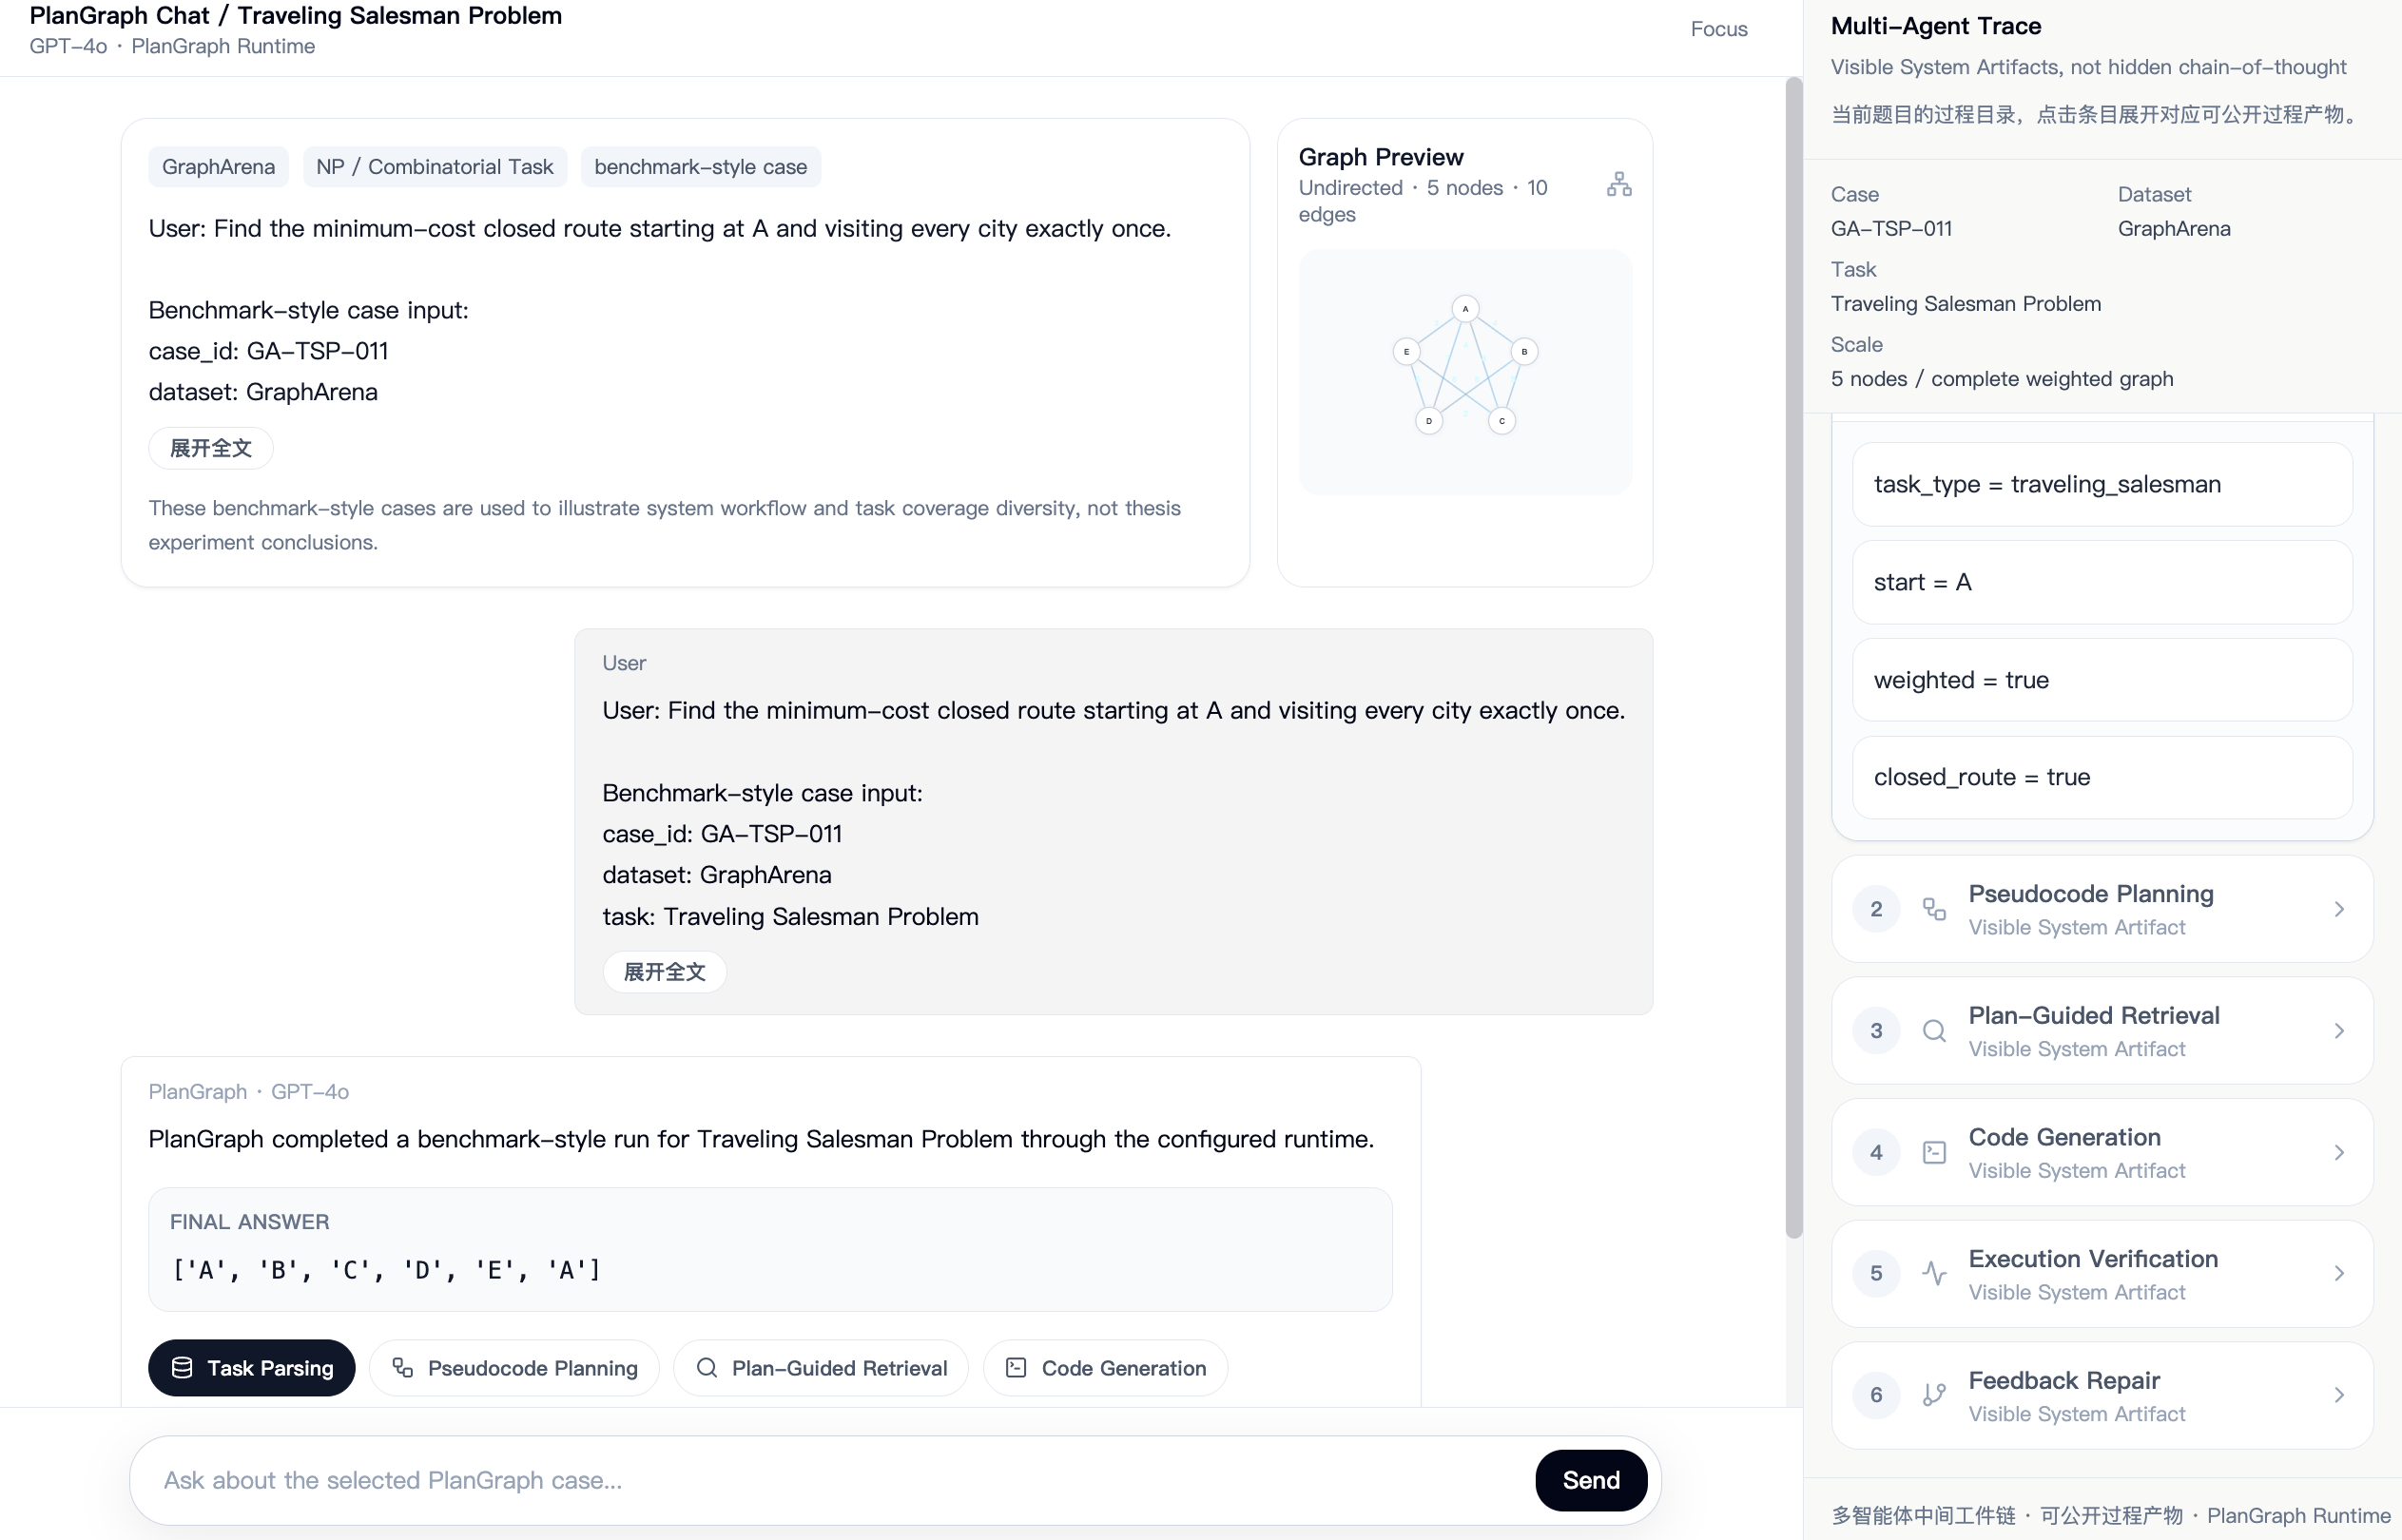
\includegraphics[width=0.95\textwidth]{figures/paper/plangraph_demo_ui.png}
    \caption{PlanGraph 协同过程展示界面}
    \label{fig:plangraph_demo_ui}
\end{figure}

展示原型仅用于呈现同一求解链路中的阶段结果，实验统计仍来自统一数据集、统一指标和批量运行日志。第四章的核心仍是黑板调度、共享缓存和反馈恢复三类机制，原型只辅助说明这些机制在单个样例中的运行过程。

\section{协同推理机制验证}
\label{sec:system_validation}

本节检验黑板调度下的协同推理机制能否稳定支撑多轮求解过程。验证重点放在三个方面：共享黑板是否能够减少状态漂移，共享缓存是否能够支撑失败回放和恢复，错误归因与预算控制是否能够降低无效重试。围绕这些问题，本文从重复运行稳定性、检索信号质量、参数预算、运行开销、鲁棒性和消融实验等方面展开验证。

\subsection{重复运行稳定性分析}

对于多智能体图推理系统而言，单次精确匹配率只能反映最终答案是否正确，还需要考察多次运行时结果是否稳定，以及候选程序在失败后能否在限定轮数内收敛。因此，本文从不同运行轮次之间的精确匹配率波动范围、程序首次生成即通过验证的比例，以及进入修复循环后能够在限定轮数内收敛的比例三个角度进行统计，结果如表\ref{tab:stability_observation}所示。

\begin{table}[htbp]
\centering
\caption{重复运行中的稳定性观察（\%）}
\label{tab:stability_observation}
\begin{tabular}{lccc}
\toprule
数据集 & 精确匹配率波动范围 & 首次通过率 & 修复后收敛率 \\
\midrule
GraphArena & $\pm0.7$ & 79.6 & 91.4 \\
NLGraph & \textbf{$\pm0.5$} & \textbf{82.3} & \textbf{93.1} \\
GraphWiz & $\pm0.9$ & 74.8 & 89.7 \\
\bottomrule
\end{tabular}
\end{table}

表\ref{tab:stability_observation}显示，结构较清晰、标准算法映射较稳定的任务在三个指标上整体更优；约束更复杂的任务首次通过率略低，但经过反馈修复后仍能保持较高收敛水平。该结果说明，PlanGraph 的协同推理机制除了提高单次运行的精确匹配率，还能抑制多次运行时的结果波动，并对失败样例提供有限恢复能力。黑板事件和共享缓存链为这些统计提供了直接依据：每次失败、修复和重新验证都被记录为可追踪事件，因此可以区分首次成功、修复成功和最终失败三类情况。

\subsection{检索质量验证}

为了更细致地验证共享黑板中的规划状态和结构约束标签是否能改善检索智能体的输入质量，本文比较四种查询方式：直接使用原始问题文本进行检索、使用任务类型和关键词进行简化检索、使用规划伪代码进行检索，以及在规划伪代码基础上补充结构约束标签进行检索。实验基于五个基准测试集构造对应查询实例，统计 Hit@1、Hit@3、Hit@5 以及平均倒数排名（MRR）四项指标，结果如表\ref{tab:retrieval_quality}所示。

\begin{table}[htbp]
\centering
\caption{不同检索查询方式的知识命中效果对比}
\label{tab:retrieval_quality}
\begin{tabular}{lcccc}
\toprule
查询方式 & Hit@1 & Hit@3 & Hit@5 & MRR \\
\midrule
Q1 原始问题文本 & 42.6\% & 61.8\% & 72.9\% & 51.4\% \\
Q2 任务类型和关键词 & 68.9\% & 84.7\% & 92.1\% & 76.3\% \\
Q3 规划伪代码 & 76.4\% & 90.8\% & 96.3\% & 83.5\% \\
Q4 规划伪代码及结构约束标签 & \textbf{82.1\%} & \textbf{94.2\%} & \textbf{98.0\%} & \textbf{88.4\%} \\
\bottomrule
\end{tabular}
\end{table}

从表\ref{tab:retrieval_quality}可见，四种查询方式呈现出清晰的层次关系：直接使用原始问题文本的效果最弱；在显式加入任务语义后，Q2 的命中效果明显提升；将问题压缩为规划伪代码后，Q3 在四项指标上继续改善；当查询中继续补充图类型、目标形式和关键约束等结构化标签时，Q4 的检索排序质量达到最好。Q3 和 Q4 在 MRR 上的提升还说明，黑板中保存的规划状态会影响正确知识的召回情况和排序位置，从而有助于减少编码阶段对错误 API 或不相关文档的尝试次数。这一结果从实验上支持了共享状态约束检索输入的协同推理机制。

\subsection{参数敏感性分析}

为观察检索返回条数和修复轮数对协同恢复过程的影响，本文比较六组代表性参数组合，即 $(1,0)$、$(3,1)$、$(5,3)$、$(7,3)$、$(5,4)$ 和 $(9,4)$。其中，$k$ 表示检索模块返回的候选知识条目数，$r$ 表示最大反馈修复轮数。该实验选取具有稳定难度分层的典型组合优化任务子集，重点比较简单样本与困难样本两个端点，并统计子集精确匹配率、难度分层精确匹配率、执行成功率、平均修复轮数与平均端到端耗时。该处数值用于分析预算约束和恢复深度，不对应第五章完整基准集合上的总体精确匹配率。

\begin{table}[htbp]
\centering
\caption{不同参数组合下典型组合优化子集的性能比较（\%）}
\label{tab:param_main_result}
\small
\resizebox{\textwidth}{!}{%
\begin{tabular}{lcccccccc}
\toprule
$(k,r)$ & 子集 EM & 简单样本 EM & 困难样本 EM & 执行成功率 & 平均修复轮数 & 平均耗时(s) & $\Delta$EM vs $(3,1)$ & $\Delta$耗时(s) vs $(3,1)$ \\
\midrule
$(1,0)$ & 70.00 & \textbf{85.00} & 55.00 & 74.20 & \textbf{0.00} & \textbf{13.80} & -4.17 & -1.40 \\
$(3,1)$ & \textbf{74.17} & 82.50 & 63.75 & 80.80 & 0.36 & 15.20 & 0.00 & 0.00 \\
$(5,3)$ & 68.75 & 75.00 & 61.25 & 78.30 & 0.92 & 18.40 & -5.42 & +3.20 \\
$(7,3)$ & 73.75 & 80.00 & \textbf{66.25} & \textbf{81.70} & 0.88 & 17.60 & -0.42 & +2.40 \\
$(5,4)$ & 71.25 & 75.00 & 65.00 & 80.40 & 1.14 & 20.90 & -2.92 & +5.70 \\
$(9,4)$ & 71.25 & 77.50 & 63.75 & 79.20 & 1.20 & 19.70 & -2.92 & +4.50 \\
\bottomrule
\end{tabular}
}
\end{table}

表\ref{tab:param_main_result}显示，$r=0$ 时 PlanGraph 缺少反馈修复能力，困难样本精确匹配率下降到 55.00\%；当参数增大到 $(7,3)$、$(5,4)$ 或 $(9,4)$ 时，更多知识条目和修复轮数未带来稳定的子集收益。相比之下，$(3,1)$ 能够在保持较高子集精确匹配率的同时控制平均修复轮数和平均耗时，说明适中的检索规模与少量反馈修复更适合作为默认配置，也说明有界恢复比无约束增加修复轮数更符合协同调度目标。

\subsection{运行开销分析}

为了说明 PlanGraph 的运行代价，本文统计了其在典型任务上的平均端到端推理耗时、平均代码生成轮数和平均验证次数。这里选取三类代表任务：最短路径、最大流和旅行商问题。平均耗时会受到模型接口响应、返回长度与验证轮次等因素影响，因此表\ref{tab:efficiency}中的数值主要用于展示本系统在不同任务之间的相对开销差异。

\begin{table}[htbp]
\centering
\caption{不同任务上的平均推理开销}
\label{tab:efficiency}
\begin{tabular}{lccc}
\toprule
任务类型 & 平均耗时（s） & 平均生成轮数 & 平均验证次数 \\
\midrule
最短路径 & \textbf{10.8} & \textbf{1.1} & \textbf{1.3} \\
最大流 & 14.6 & 1.3 & 1.8 \\
旅行商问题 & 24.3 & 1.8 & 2.7 \\
\bottomrule
\end{tabular}
\end{table}

表\ref{tab:efficiency}显示，不同任务的运行开销差异较明显。最短路径问题结构相对清楚，算法接口也较成熟，因此规划、检索和验证过程通常较为顺畅。最大流任务需要处理容量约束和残量网络，程序实现中涉及的状态更新更多，平均验证次数因此有所增加。旅行商问题还需要显式处理组合搜索、节点覆盖、回路闭合和可行性判断，因而整体耗时和验证次数最高。就本文研究目标而言，更强调可靠地完成图推理，而非追求最低时延响应，因此以一定推理开销换取更高精确匹配率和结果可信度是合理的设计选择。

\subsection{鲁棒性消融分析}

除标准基准测试集外，本文还在输入扰动设置下考察 PlanGraph 的表现，以分析框架对问题表述变化的稳定性。该实验覆盖五个基准测试集，并构造三种常见扰动：节点顺序随机打乱、边列表描述改写、输出要求从自然语言答案改为结构化列表。在相同求解任务下比较精确匹配率变化，结果如表\ref{tab:robustness}所示。

\begin{table}[htbp]
\centering
\caption{输入扰动条件下的鲁棒性分析（\%）}
\label{tab:robustness}
\begin{tabular}{lccc}
\toprule
扰动类型 & GPT-4o & GraphTeam & PlanGraph \\
\midrule
节点顺序打乱 & 51.6 & 92.4 & \textbf{96.8} \\
边描述改写 & 48.9 & 91.1 & \textbf{95.7} \\
输出格式切换 & 44.3 & 89.8 & \textbf{94.9} \\
\bottomrule
\end{tabular}
\end{table}

表\ref{tab:robustness}显示，PlanGraph 在输入扰动下仍然保持较高精确匹配率。本文认为其原因在于：问题智能体先将自然语言输入规整为结构化表示，减少了不同表述形式对后续规划的影响；程序执行结果在最终答案生成前还会经过格式化处理，因此输出形式变化对系统影响相对有限。

为判断关键协同组成是否具有必要性，本文设计三种消融变体：（1）去除规划模块，直接根据原始问题生成代码；（2）去除检索模块，移除规划引导检索，仅依赖模型内部知识生成程序；（3）去除验证模块，移除程序执行验证与反馈修复闭环，仅保留一次性代码生成。图\ref{fig:ablation_result_visual}给出了在三个代表性数据集上的消融结果。

\begin{figure}[htbp]
\centering
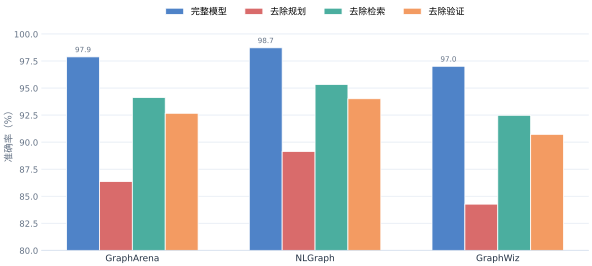
\includegraphics[width=0.90\textwidth]{figures/paper/exp_ablation.pdf}
\caption{关键协同组成消融实验结果}
\label{fig:ablation_result_visual}
\end{figure}

图\ref{fig:ablation_result_visual}显示，移除规划模块后，三个数据集上的结果都出现了最明显的下降，说明规划模块是 PlanGraph 中较关键的组成部分。去除验证模块后，系统性能也出现了较大下降，尤其在 GraphWiz 上从 97.01\% 降至 90.72\%。检索模块带来的性能提升相对温和，但依然稳定。规划模块约束任务目标与求解方向，检索模块补充实现依据，验证模块检查结果是否满足要求，三类组成形成 PlanGraph 的协同闭环。

\subsection{提示词查询模板复现说明}

为保证系统可复现性，本文将各智能体提示词和检索查询模板设计为相对固定的结构化模板。问题智能体用于将原始自然语言问题解析为结构化图推理任务，输出字段包括 \texttt{task\_type}、\texttt{nodes}、\texttt{edges}、\texttt{directed}、\texttt{weighted}、\texttt{capacity}、\texttt{params}、\texttt{output\_format} 和 \texttt{constraints}。规划智能体用于生成算法级伪代码规划，并为检索阶段提供算法提示、约束标签和检索术语。编码智能体基于任务、规划和检索知识生成可执行 Python 程序，并要求使用标准库和 NetworkX 完成图结构建模和算法调用。推理智能体则根据执行反馈和检索反馈修正当前程序，主要处理图构建错误、API 使用错误、约束遗漏和输出格式不匹配等问题。

检索智能体根据规划结果和反馈信息组织检索查询，不生成自然语言回答。其查询构造主要利用任务类型、图属性、算法提示、约束标签、输出格式以及执行错误信息。表\ref{tab:retrieval_query_template}给出了检索查询模板摘要。

\begin{table}[htbp]
\centering
\small
\caption{检索查询模板摘要}
\label{tab:retrieval_query_template}
\begin{tabular}{p{2.0cm}p{10.5cm}}
\toprule
查询类型 & 构造依据 \\
\midrule
\texttt{Q0} & \texttt{task\_type and graph attributes} \\
\texttt{Q1} & \texttt{key actions from pseudocode and algorithm\_hints} \\
\texttt{Q2} & \texttt{constraint\_tags and output\_format} \\
\texttt{Q3} & \texttt{retrieval gaps or low-coverage constraints} \\
\texttt{Q4} & \texttt{execution error type, failed API, and repair target} \\
\texttt{Ranking} & \texttt{semantic relevance, task-tag matching, and constraint consistency} \\
\bottomrule
\end{tabular}
\end{table}

上述模板避免暴露模型内部不可控推理链，并要求各阶段返回可检查的阶段结果。通过固定字段、固定查询类型和统一输出格式，PlanGraph 能够在批量实验中保持较一致的运行条件，也便于对失败样例进行回放和复核。


\section{本章小结}

本章围绕多智能体图推理中的协同推理机制展开，重点研究规划、检索、编码、验证和修复等角色如何在统一状态约束下完成一条可追踪、可恢复和可复现的求解链路。核心问题包括多个智能体如何共享状态、如何依据错误来源选择恢复动作，以及如何通过运行记录支撑机制分析。

首先，本章提出基于共享黑板的协同状态建模机制，用 $B_t=\{Q,S,P,K,C,E,F,A\}$ 描述原始问题、结构化任务、规划结果、检索知识、候选程序、执行验证、反馈修复和最终答案之间的状态关系，并通过黑板事件约束角色智能体和功能模块的读写边界。其次，本章提出基于错误归因的协同调度机制，将执行观测、错误类型和剩余预算纳入调度策略，使系统能够在局部修复、补充检索、重新规划、重生成和失败退出之间进行有依据的选择。再次，本章提出基于共享缓存的反馈恢复机制，通过缓存版本、依赖关系和运行产物管理保留阶段结果，使失败样例能够被定位、回放和复核。最后，本章通过运行记录诊断机制记录黑板快照和约束验证反馈，使协同推理过程具有可观察的研究证据。

协同推理机制验证表明，黑板事件和缓存版本能够保留阶段依赖，预算控制能够限制无效重试，反馈恢复能够提高失败样例的收敛比例。重复运行稳定性、检索信号质量、参数敏感性、运行开销、鲁棒性和消融实验进一步说明，第四章所述机制能够将多智能体协作约束为状态一致、错误可归因和恢复有边界的协同推理过程。这为后续评价完整 PlanGraph 框架的总体效果提供了运行层依据。
